% Set the author and title of the compiled pdf
\hypersetup{
  pdftitle = {\Title},
  pdfauthor = {\Author}
}

\section{Setting the stage}

Before it is possible to understand some of the content in these notes, it is
required to have a basic knowledge of other content that was not covered in my
previous notes. This section attempts to give an overview of the relevant
topics.

\subsection{Decision problems}

A decision problem is essentially a question, described by some formal language
(such as that of propositional logic) with a yes/no answer. In order to obtain
whether the decision problem yields yes or no, input parameters must be
specified and the problem evaluated according to the language it is written in.

Another requisite of a decision problem is that the possible set of inputs must
be infinite. That is to say that $5 = 5$, or ``Is the sky blue?'' would not be a
decision problem, since the set of inputs in both cases is the $\emptyset$.
Likewise, if a problem doesn't yield a yes/no answer (for example, a quadratic
equation), then it is not a decision problem.

\subsubsection{Decidable problems}

A problem is classed as decidable if it is both a decision problem and there
exists and algorithm that will be able to compute the correct answer for all
(infinite number of) inputs to the problem. Such an algorithm can be described
by any Turing complete programming language, in fact, it works both ways; if
there is a computer program which can find the correct yes/no answer for a
decision problem over all inputs, then the problem must be decidable.

Some decision problems are undecidable. It is impossible to create an algorithm
that can always solve the problem for all of its inputs. One such problem is the
Halting problem, which asks:

\begin{quotation}
  Given the description of an arbitrary program and a finite input, decide
  whether the program finishes running or will run forever.
\end{quotation}

It has been proven that the Halting problem is undecidable when running on a
Turing machine. The essence of the proof is that the algorithm evaluating
whether the input program will halt or not could be made to contradict itself.

\subsection{Mappings}

A mapping is a function that takes an input from one set and returns an output
from another (or the same) set. Conversely, you could describe a function as
mapping one set to another.

The notation $ f'(x) = f(x) + \{ a \rightarrow b\}$ means:

\[
  f'(x) \definedas
  \begin{cases}
    b    & \text{if x = a}\\
    f(x) & otherwise
  \end{cases}
\]

\subsection{Binary relations}

Binary relations are often denoted by $\Rightarrow$, and it's reverse is denoted
by $\Leftarrow$ such that $y \Leftarrow x \definedas x \Rightarrow y$. Along a
similar train of thought, the symmetric closure of $\Rightarrow$ is
$\Leftrightarrow$, where $\Leftrightarrow \definedas \Rightarrow \cup
\Leftarrow$

\subsection{Orders}

An order is a relation that is irreflexive and transitive. This means that each
pair in the relation cannot be constructed of only one element (e.g. $x > x$
wouldn't be allowed) and if $((x > y) \wedge (y > z)) \implies x > z$.

\subsection{Directed graphs}

A directed graph consists of a set $N$ and a binary relation on the set $R$. The
elements in $N$ are nodes, and the relation $R$ defines the edges between the
nodes. A directed graph is finite if it's set is finite.

A \textit{path} is a subset of $R$ where each element of the path will end at
the start of another element with the exception of the start and end elements. A
cycle is a path where there is no start and end pairs.

\subsubsection{Directed Acyclic Graphs (DAG's)}

A Directed Acylcic Graph is a directed graph that has no cycles. If a dag has a
node $n$ such that every other node in the dag is reachable by $n$, then the dag
is \textit{rooted at $n$}.


\section{Propositional logic}

Thankfully, we covered propositional logic in some detail in the COMP11120
course in the first year. However, this module builds upon what was learnt in
the first year, and so there is more to learn!

This course introduces the idea of an \textit{interpretation}. An interpretation
of a propositional formula is the values that are assigned to each variable in
the formula. Assigning values to variables should be a familiar concept,
however, calling it an interpretation brings the idea closer to the real world
since the formula can be interpreted to mean something in a specific context.
Interpretations are also referred to as truth assignments, and boolean values
are referred to as truth values.

In this course, we sometimes need to assign a truth value to an expression that
contains a conjunction or disjunction and nothing more. If this is the case,
then for every interpretation, conjunctions evaluate to true, and disjunctions
evaluate to false.

There is a notation to generalise the fact that an interpretation may be a model
of many different formulas. If $S$ is a set of formulas for which an
interpretation $I$ is a model, then:

\[
  I \models S
\]

If two formulas can be modelled by exactly the same interpretations, then they
are said to be \textit{equivalent}, the symbol for which is $\equiv$.

For a summary of the above couple of paragraphs, look at the properties in
Table~\ref{table:PL-laws}.

\marginpar{`iff' means `if and only if'}

\begin{table}[!h]
  \centering
  \begin{tabular}{l}
    \multicolumn{1}{c}{\textbf{Property}}\\ \hline
    $A$ can only be valid if $\neg A$ is unsatisfiable.\\
    $A$ can only be satisfiable iff $\neg A$ is not valid.\\
    $A$ is valid iff $A \equiv \top$.\\
    $A \equiv B$ iff $A \Leftrightarrow B$.
  \end{tabular}
  \label{table:PL-laws}
  \caption{Some of the fundamental properties of PL}
\end{table}

\subsection{Subformulae}

A subformula is essentially a formula within a formula. Every formula is
composed of one or more subformulae and every formula is it's own subformula.

Imagine that a formula is composed of layers, with each layer being composed of
an operator (such as a number of conjunctions, or an implication). The immediate
subformulae of a formula is the components that the outermost layer uses. It's a
hard thing to describe using an informal language such as English, so here are
some more concrete examples:

\begin{itemize}
  \item $A_1 \dots A_n$ are immediate subformulae of
        $A_1 \vee \dots \vee A_n$, and $A_1 \wedge \dots \wedge A_n$.
  \item The formula $A$ is an immediate subformula of $\neg A$.
  \item $A_1\text{~and~}A_2$ are immediate subformulae of $A_1 \Rightarrow A_2$
        and $A_1 \Leftrightarrow A_2$.
  \item Every formula is a subformula of itself.
  \item If $A_1$ is an immediate subformula of $A_2$, and $A_2$ is an immediate
  subformula of $A_3$, then $A_1$ is a \textbf{subformula} of $A_3$.
\end{itemize}

The above table and previous discussions of equivalence mean that if we replace a
subformula $A$ in a formula $X$ by another subformula $B$ that is equivalent to
$A$ ($A \equiv B$), to give $Y$, then $X \equiv Y$.

\section{Evaluating formulae}

Evaluating formulae can be viewed as a decision problem. If a formula under a
specific interpretation is true, then the answer is \textit{yes}, otherwise it's
\textit{no}.

It is possible to evaluate formulae relatively efficiently by evaluating each
immediate subformula in turn. For example, if we wanted to evaluate the
expression $a \Rightarrow b$, we would evaluate $b$ first, since if $b \equiv
\top$, then the whole expression would evaluate to $\top$. Only in the case
where $b \equiv \bot$, would we need to evaluate $a$.

This method of evaluating formulae can be done cleanly using a table such as the
one in Table~\ref{table:evaluate}.

\begin{table}
  \centering
  \begin{tabular}{l >{$}c<{$} l}
      & Subformula & Value\\ \hline
    1 & (p \implies q) \wedge (p \wedge q \implies r) \implies (p \implies r) & 1\\
    2 & \phantom{(p \implies q) \wedge (p \wedge q \implies r) \implies }(p \implies r) & 1\\
    3 & (p \implies q) \wedge (p \wedge q \implies r) \implies \phantom{(p \implies r)} & 0\\
    4 & \phantom{(p \implies q) \wedge} (p \wedge q \implies r) \phantom{\implies (p \implies r)} & 1\\
    5 & (p \implies q) \phantom{\wedge (p \wedge q \implies r) \implies (p \implies r)} & 0\\
    6 & \phantom{(p \implies q) \wedge (}p \wedge q \phantom{\implies r) \implies (p \implies r)} & 0\\
    7 & \phantom{(}p\phantom{\implies q) \wedge (}p\phantom{\wedge q \implies r) \implies (}p\phantom{ \implies r)}& 1\\
    8 & \phantom{(p \implies }q\phantom{) \wedge (p \wedge }q\phantom{ \implies r) \implies (p \implies r)} & 0\\
    9 & \phantom{(p \implies q) \wedge (p \wedge q \implies }r\phantom{
    ) \implies (p \implies }r\phantom{)} & 1\\
  \end{tabular}
  \label{table:evaluate}
\end{table}

\subsection{Rewrite rules}

It is possible to evaluate a formula simply by rewriting the subformulae inside
of it. In order to do this, replace each atom in the formula by it's truth value
in the interpretation:

For $A = (x \vee y) \implies z$, and $I = \{x \rightarrow 0, y \rightarrow 1, z
\rightarrow 0\}$:

\[
  (x \vee y) \implies z
\]
\[
  (\bot \vee \top) \implies \bot
\]

Then we can use the PL rewrite rules to iterate towards a final truth value:

\begin{align}
  (\bot \vee \top) \implies &\bot \equiv \top \implies \bot\\
  \top \implies &\bot \equiv \bot\\
  &\boldsymbol{\bot}
\end{align}

It would be very easy to write an algorithm to evaluate formulae using the
rewrite rules. Assuming a formula could be represented as a sensible
datastructure such as a tree, the algorithm needs to do the following steps:

\begin{enumerate}
  \item Traverse the formula and replace all atoms by their values in the
        current interpretation.
  \item While the formula is not $\top$ or $\bot$, re-write the formula using
        the re-write rules
  \item Return either $\top$ or $\bot$
\end{enumerate}

\subsection{Circuits}

% TODO: Is isomorphic the right word here?

There exists a certain isomorphism between PL and digital circuitry. It is
often possible to reduce a problem of digital logic (one that involves the use
of AND, OR, XOR and other gates) into one that can be represented by a PL
formula.

Though this may seem both trivial and frivolous at first, there exist many good
reasons for such an exercise. For example, it would be possible to check if two
circuits did the same thing using techniques from PL, or you could use re-write
rules to make one circuit into another equivalent, yet more compact circuit.

\section{Satisfiability}

Checking if a PL formula is satisfiable (there is at least one interpretation
where the formula is true) is a famous decision problem.

The satisfiability problem is NP-Complete (so we can check the solution quickly,
but we cannot arrive at the solution in polynomial time).

One simple way of checking the satisfiability of a formula is to enumerate all
the possible interpretations, and put them in a truth table. As usual, you split
the formula into it's subformulae, but unlike a conventional truth table, you
have a column for each interpretation (so enumerate the possible combinations of
all the atomic formulae).

Using truth tables as a method of satisfiability checking is not very
efficient. Because there is a requirement to enumerate all of the
interpretations, you need to do as many operations as there are $2^{\#atoms}$.

When you think about it, there will be certain situations, where we don't have
to enumerate all of the different interpretations. For instance if we assume
that $I(r) = \top$, then we know that $I(p \vee r) = \top$ and $I(x \implies (p
\vee r)) = \top$. In this example, we could eliminate lots of possible
interpretations since we know some of them to be valid without even trying them.

If we were to take this principle into account when evaluating formulae for
satisfiability, how many enumerations we would need to do would depend on which
variables we enumerated first. Good SAT checkers will choose wisely in this
regard.

\subsection{Signed Formulae}

In order to progress, we need to understand the notion of signed formulae.

A signed formula, $A = b$ is one where the formula $A$ is equal to $b$ in a
specific interpretation $I$. It follows that:

\begin{itemize}
  \item For any $A$ and any $I$ either $A = 1$ or $A = 0$ in $I$.
  \item The formula $A$ is satisfiable iff $A = 1$
\end{itemize}

\subsection{Splitting}

Splitting is another way of checking satisfiability of formulae. The idea is
that we consider truth values for variables in the formula, and simplify the
formula based on those considerations. Formally:

\textit{For every propositional formula $A$, and every atom $p$, denote
$A^{\top}_p$ and $A^{\bot}_p$ as the formulas with $p$ replaced with $\top$ and
$\bot$ respectively.}

The splitting algorithm tells us if each interpretation of a formula is
satisfiable or unsatisfiable. If all the interpretations are $\top$, then the
formula must be valid, if they are all $\bot$, then it must be unsatisfiable.

Figure~\ref{fig:andrei-split}, (the same example used in Andrei's notes) shows
the splitting algorithm in action. I think its easiest to learn splitting
through diagrams such as this, and thus I won't write any more about how it
works.

\begin{figure}[!h]
  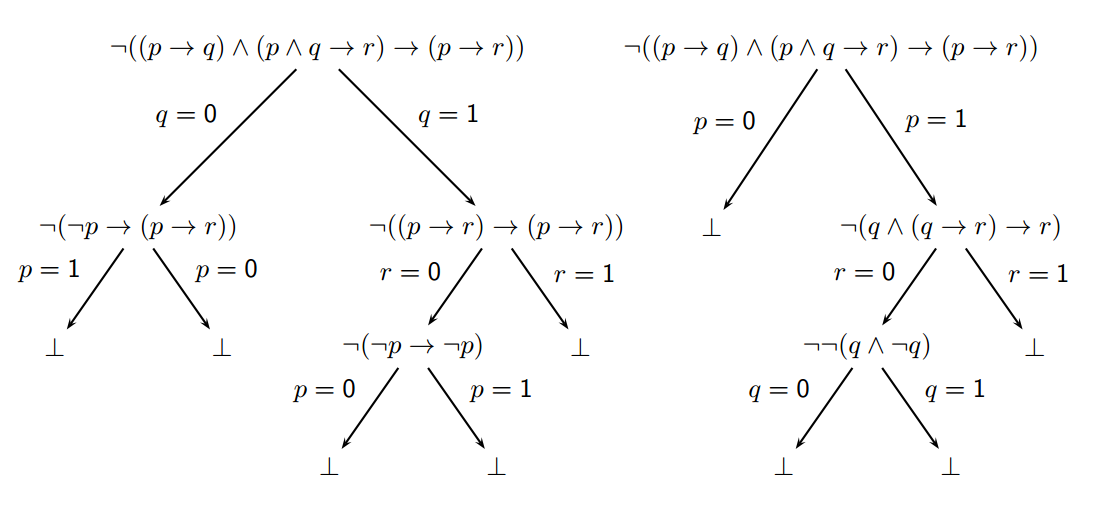
\includegraphics[width=\textwidth]{diagrams/andrei-splitting}
  \caption{Splitting the formula $\neg((p \implies q) \wedge (p \wedge q \implies r) \implies (p \implies r))$}
  \label{fig:andrei-split}
\end{figure}

\subsection{Polarity of subformulae}

\section{CNF}

\section{Definitional Clausal Form Translation}

\section{DPLL}

\section{Encoding problems in SAT}

\section{Randomly generated clause sets}

\section{Randomised algorithms for satisfiability checking}

% Lecture 10
\section{Signed Formulae}

A signed formula is one where there is an expression, $A$ and a boolean $b$,
where $A = b$. If $A = b$ is {\it true}, in an interpretation $I$, then it is
denoted by $I \models A = b$, and consequently, $I$ is a model of the signed
formula $A = b$.

\marginpar{This is also when $I(A) =b$.}

If a signed formula has a model, then it is specifiable.

\subsection{Finding a model of a specifiable formula}

If we had a signed formula such as $A \Leftrightarrow B = 1$, the three
interpretations that model it are:

\begin{center}
    \begin{tabular}{cc}
        A & B\\ \hline
        0 & 0\\
        0 & 1\\
        1 & 1\\
    \end{tabular}
\end{center}

\subsection{Tabelau}

A tableau is a tree with each node being a signed formula. The tableau for the
signed formula $A = b$ would have the root node as $A = b$.

The notation for a set of branches is $B_1 | ... | B_n$, where each $B_i$ is a
branch.

\subsubsection{Branch expansions}

There are a number of rules that can be used to expand the branches of a
tableau.
